\subsection{Implementación en PCB}

Una vez definidos todos los circuitos que componen a la plataforma, se llega a un total de {\Medium 185 componentes} discretos con decenas de empaquetados distintos, que deben todos ser posicionados en una placa de circuito impreso doble faz del menor tamaño posible. El resultado final de la plaqueta, con todos sus componentes (exceptuando los disipadores térmicos de los transistores y diodos de potencia) se observa en la figura \ref{fig:PCB_3D}.\\

\begin{figure}[h]
    \centering
    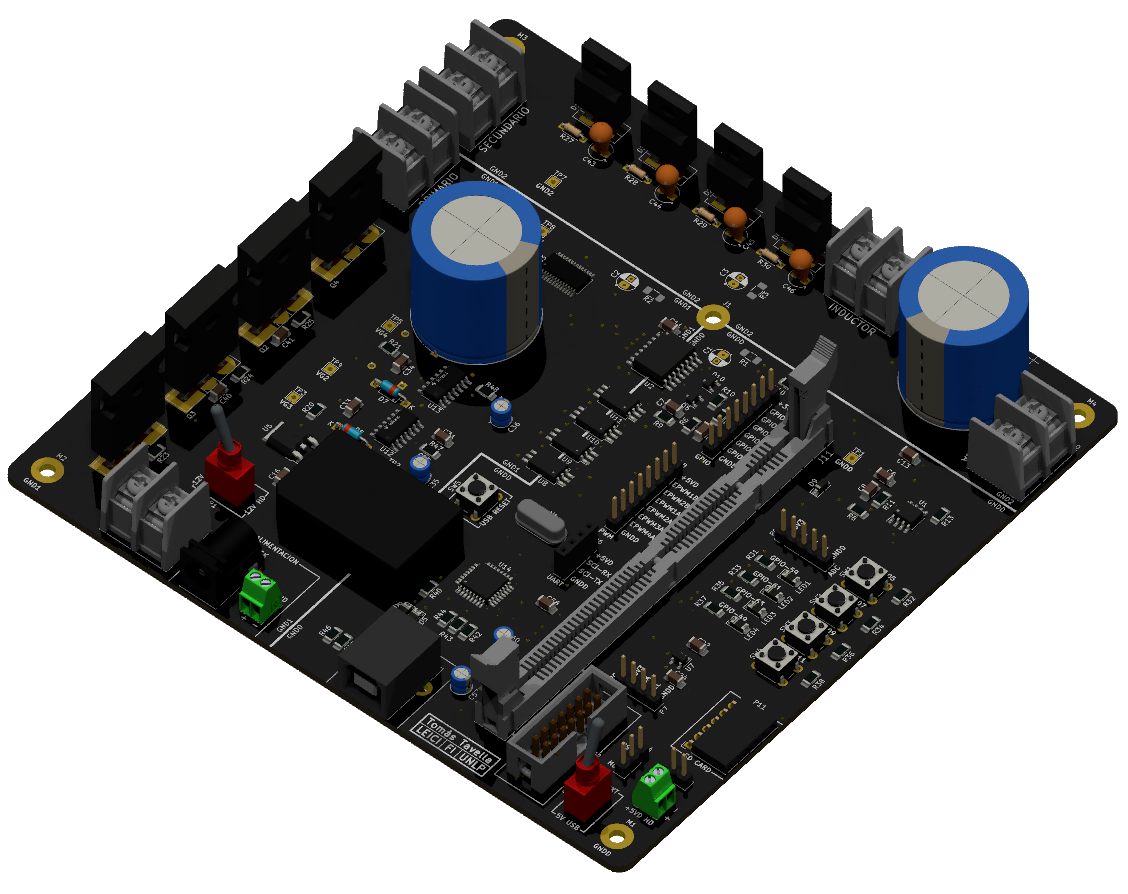
\includegraphics[scale=0.32]{Imagenes/PCB 3D Raytracing.png}
    \caption{Modelo tridimensional de la implementación en PCB de la plataforma con todos sus componentes, vista desde la parte superior.}
    \label{fig:PCB_3D}
\end{figure}

Para comenzar, se va a realizar un listado de todos los componentes, clasificados según sus distintos encapsulados y sus \textit{footprints} correspondientes (es la \quotes{huella} de cada componente sobre la plaqueta), para luego detallar el proceso por el que se posicionaron y conectaron sobre la PCB.\\

\subsubsection{Listado de Componentes}

\lipsum[1]\\

\setlength{\tabcolsep}{8pt}
\renewcommand{\arraystretch}{1.5}
\begin{table}[h]
\begin{center}
    \begin{tabular}{llrrr}
        {\SemiBold Tipo} & {\SemiBold Dispositivo} & {\SemiBold Tensión} [\unit{\volt}] & {\SemiBold Corriente} [\unit{\milli\ampere}] & {\SemiBold Total} [\unit{\milli\ampere}]\\
        \hline
        \multirow{4}{*}{Potencia} & 2ED21834-S06J (x2) & \num{10}-\num{20} & 2200 & 2200\\
        \cline{2-5}
         & ACPL-P480 (x4) & \num{5} & \num{12} & \multirow{3}{*}{43.5} \\
         & LM5056A & \num{5} & \num{7.5} & \\
         & ISO7242C (Lado 1) & \num{5} & \num{24} & \\
        \hline
        \multirow{4}{*}{Digital} & TMCS1100A4 & \num{5} & \num{6} & \multirow{3}{*}{331} \\
         & TMS320F28335 & \num{5} & \num{300} & \\
         & FT232BL & \num{5} & \num{25} & \\
         \cline{2-5}
         & ISO7242C (Lado 2) & \num{3.3} & \num{24} & 24
    \end{tabular}
    \caption{Listado de los distintos encapsulados y footprints de todos los componentes de la placa. (Placeholder)}
    \label{tabla:footprints}
\end{center}
\end{table}

\lipsum[2]\\

\newpage\afterpage{\blankpage}

\begin{figure}[H]
    \centering
    \subfigure[Capa de cobre frontal, con los distintos bloques de la plataforma indicados.]{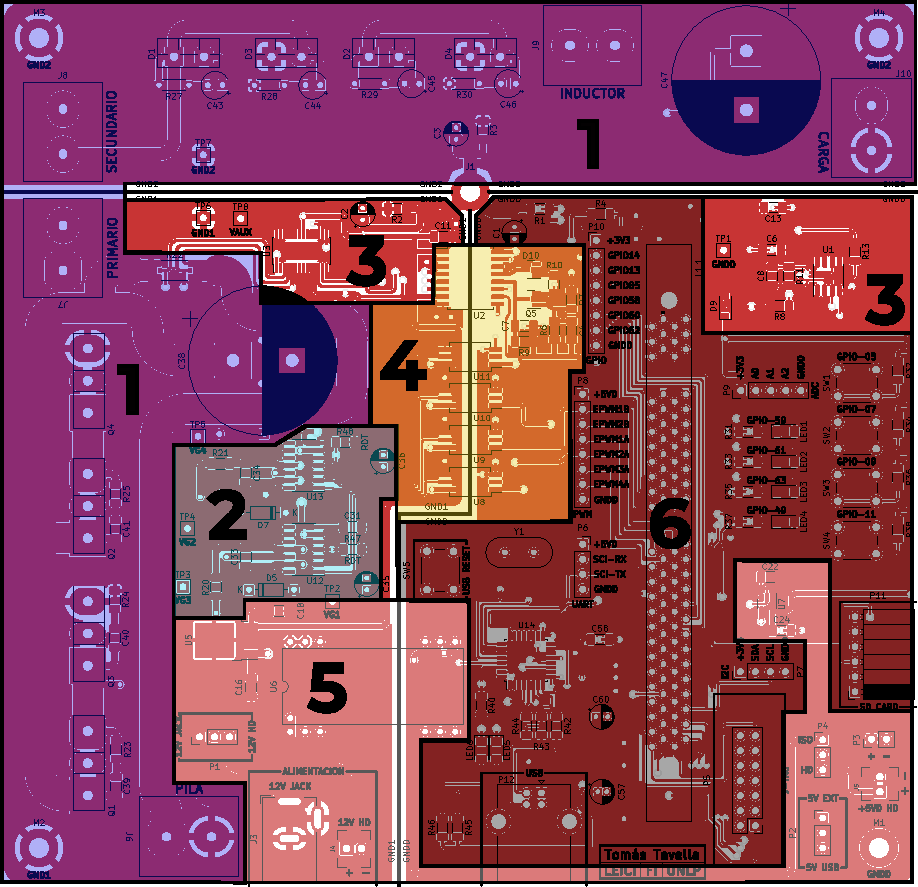
\includegraphics[scale=0.8]{Imagenes/PCB Front - SubCircuitos.pdf}}\\
    \subfigure[Capa de cobre trasera, con las tres distintas puestas a tierra.]{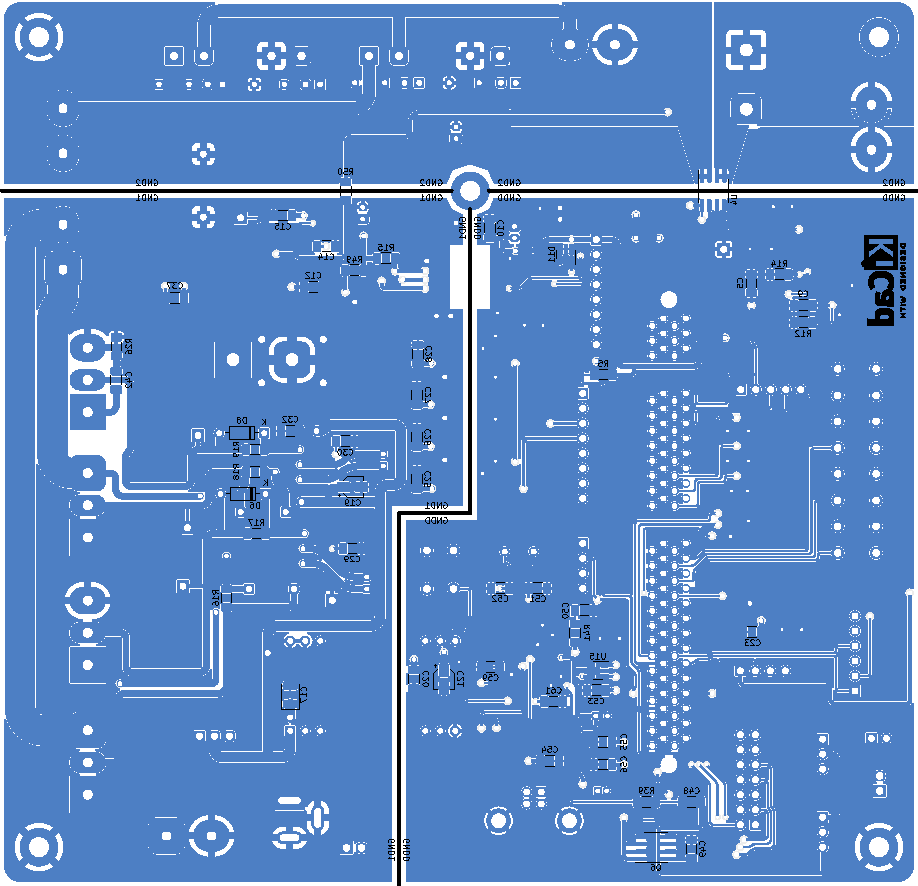
\includegraphics[scale=0.8]{Imagenes/PCB Back Layer.pdf}}%
    \caption{Diagrama de las distintas capas de cobre de la PCB.}
    \label{fig:PCB_cobre}
\end{figure}